\section{Introduction}
\label{Introduction}

Consider the discrete-time linear system dynamical process model and linear observation model

\begin{equation*}
    \begin{aligned}
        \mathbf{x}_{k+1} &= \mathbf{\Phi}_{k+1|k} \mathbf{x}_k + \mathbf{u}_k + \mathbf{\Gamma}_{k+1|k} \mathbf{w}_k \\
        \mathbf{z}_k &= \mathbf{H}_k \mathbf{x}_k + \mathbf{v}_k
    \end{aligned}
\end{equation*}

where $\mathbf{x}$ is an $n \times 1$ state vector,
$\mathbf{\Phi}$ is an $n \times n$ state transition matrix,
$\mathbf{u}$ is an $n \times 1$ control input,
$\mathbf{\Gamma}$ is an $n \times p$ disturbance distribution matrix,
and $\mathbf{w}$ is a $p \times 1$ white process noise sequence of random disturbances with covariance

\begin{equation*}
    \mathbf{Q}_k = E \left\{ \mathbf{w}_k \mathbf{w}_k^T \right\}
\end{equation*}

and where $\mathbf{z}$ is an $m \times 1$ observation vector,
$\mathbf{H}$ is an $m \times n$ observation transformation matrix,
and $\mathbf{v}_k$ is an $m \times 1$ white error noise sequence of random observation errors with covariance

\begin{equation*}
    \mathbf{R}_k = E \left\{ \mathbf{v}_k \mathbf{v}_k^T \right\}
\end{equation*}

and where both the process and observation noise sequences are uncorrelated

\begin{equation*}
    E \left\{ \mathbf{w}_j \mathbf{v}_k^T \right\} = \mathbf{0} \, , \phantom{.} \mathrm{for} \, \mathrm{all} \, j \, \mathrm{and} \, k
\end{equation*}

Figure \ref{fig:dt-linear-system} diagrammatically depicts the linear system model.

\begin{figure}[ht]
    \centering
    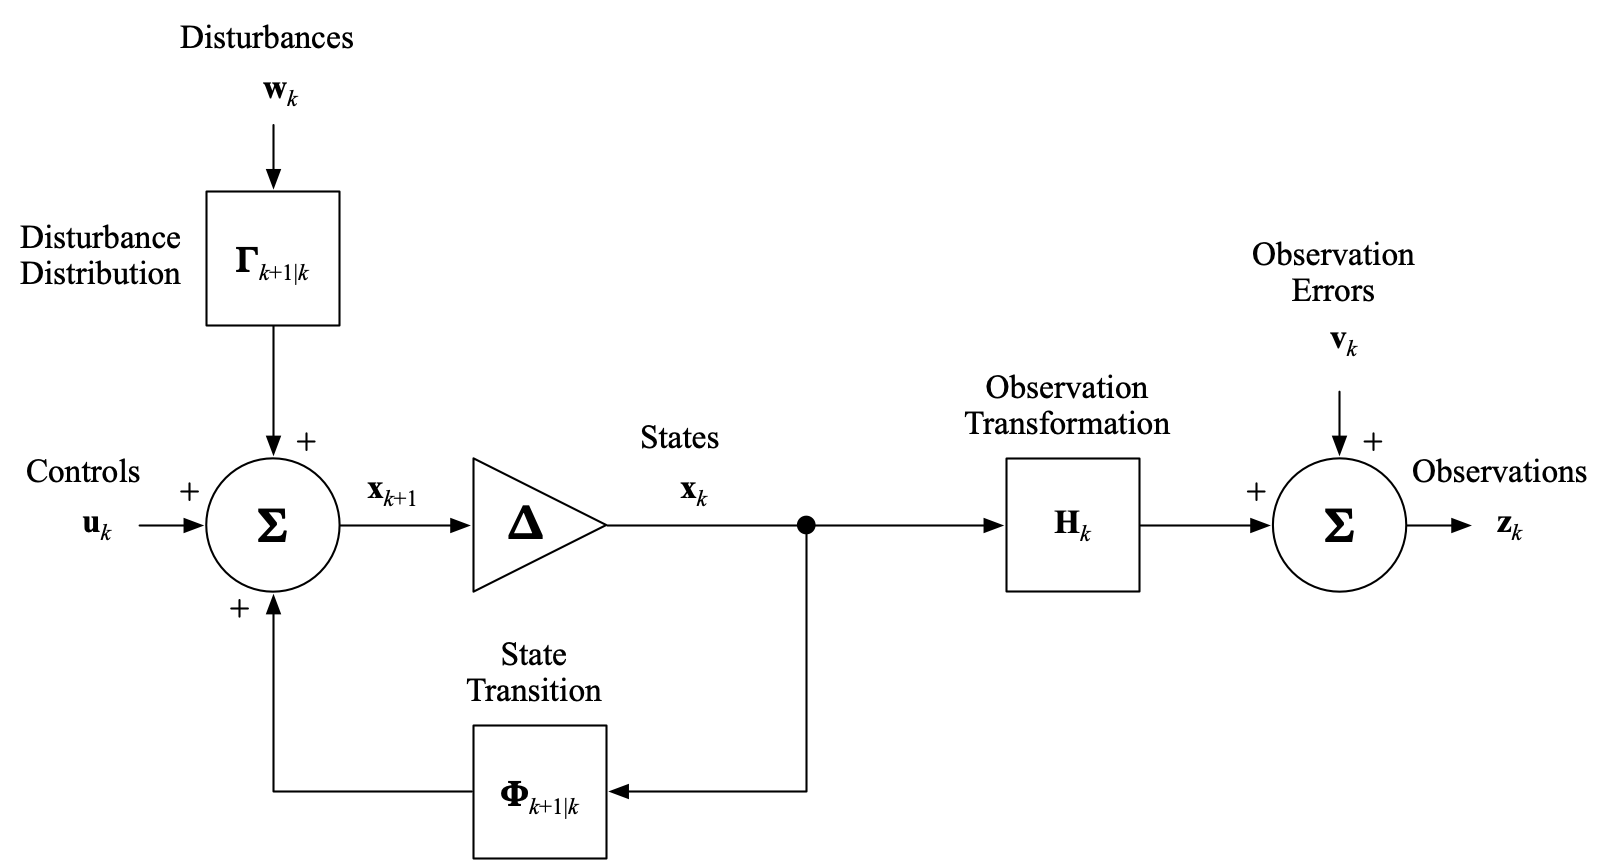
\includegraphics[width=0.95\textwidth]{images/DT-Linear-System.png}
    \caption{Discrete-Time Linear System}
    \label{fig:dt-linear-system}
\end{figure}

Given the observations, $\mathbf{z}_k$,
the modeling knowledge of $\mathbf{\Phi}_{k+1|k}$, $\mathbf{\Gamma}_{k+1|k}$, and $\mathbf{H}_k$,
and the statistical characteristics of $\mathbf{w}_k$ and $\mathbf{v}_k$,
the Kalman filter provides an optimal estimate of the state, $\mathbf{x}_k$, at time event $k$

\begin{equation*}
    \hat{\mathbf{x}}_k = E \left\{ \mathbf{x}_k \right\}
\end{equation*}

with a state estimation error

\begin{equation*}
    \mathbf{e}_k = \mathbf{x}_{k} - \hat{\mathbf{x}}_k
\end{equation*}

and where the covariance of the state estimation error is

\begin{equation*}
    \begin{aligned}
        \mathbf{P}_k &= E \left\{ \mathbf{e}_k \mathbf{e}_k^T \right\} \\
        &= E \left\{ \left[ \mathbf{x}_{k} - \hat{\mathbf{x}}_k \right] \left[ \mathbf{x}_{k} - \hat{\mathbf{x}}_k \right]^T \right\}
    \end{aligned}
\end{equation*}

The well-known Kalman filter \cite{kalman1960} recurrence update cycle is comprised of two steps:
a "projection" or \textit{a priori} update, and a "correction" or \textit{a posteriori} update.

I. Projection (\textit{a priori}) update:

\begin{equation*}
    \begin{aligned}
        \hat{\mathbf{x}}_{k|k-1} &= \mathbf{\Phi}_{k|k-1} \hat{\mathbf{x}}_{k-1} + \mathbf{u}_{k-1} \\
        \mathbf{P}_{k|k-1} &= \mathbf{\Phi}_{k|k-1} \mathbf{P}_{k-1} \mathbf{\Phi}_{k|k-1}^T + \mathbf{\Gamma}_{k|k-1} \mathbf{Q}_{k-1} \mathbf{\Gamma}_{k|k-1}^T
    \end{aligned}
\end{equation*}

II. Correction (\textit{a posteriori}) update:

\begin{equation*}
    \begin{aligned}
        \hat{\mathbf{z}}_k &= \mathbf{H}_k \hat{\mathbf{x}}_{k|k-1} \\
        \tilde{\mathbf{z}}_k &= \mathbf{z}_k - \hat{\mathbf{z}}_k \\
        \mathbf{S}_k &= \mathbf{H}_k \mathbf{P}_{k|k-1} \mathbf{H}_k^T + \mathbf{R}_k \\
        \mathbf{K}_k &= \mathbf{P}_{k|k-1} \mathbf{H}_{k}^T \mathbf{S}_k^{-1} \\
        \hat{\mathbf{x}}_k &= \hat{\mathbf{x}}_{k|k-1} +\mathbf{K}_k \tilde{\mathbf{z}}_k \\
        \mathbf{P}_k &= \left[ \mathbf{I} - \mathbf{K}_k \mathbf{H}_k \right] \mathbf{P}_{k|k-1}
    \end{aligned}
\end{equation*}

Figure \ref{fig:kf-diagram} diagrammatically depicts the Kalman filter.

\begin{figure}[ht]
    \centering
    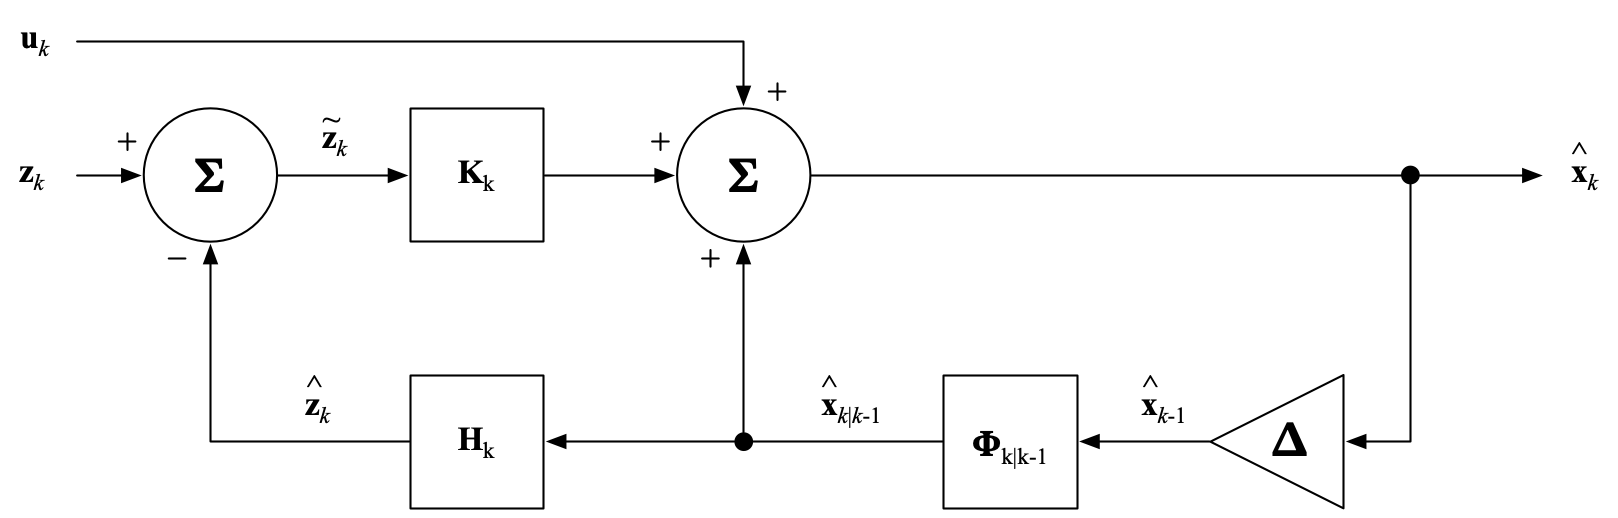
\includegraphics[width=0.95\textwidth]{images/KF-Diagram.png}
    \caption{Kalman Filter Diagram}
    \label{fig:kf-diagram}
\end{figure}

Unfortunately, the vast literature for the Kalman filter, and its varieties, can be
overwhelmingly confounding. Different variables are used. Different notations are used.
Different terms are used. The complexity of some of the mathematical proofs and theorems
can obscure the more important matters.

And then there are questions \ldots many questions.
What’s with all these equations?
What makes them so special?
Where do they come from?
What is meant by "optimal" gain?
Why can’t I just use least-squares estimation?
Isn’t the Kalman filter just a specialized least-squares filter anyway?
What does it mean when it is said that "$\mathbf{S}_k$" represents the covariance of the observation error?
Why are there so many different forms of the filter, and which one should I use?
And did Jeffrey Epstein really kill himself?

This document is an assorted collection of derivations and notes pertaining to the Kalman
filter. They are targeted to the practicing engineer who has been tasked with developing
and implementing a Kalman filtering solution. The mathematical derivations are therefore
intended to eliminate some of the mysteries of how and why the Kalman filter works, as
well as what the various versions and implementation strategies have to offer.

Some assumptions are made about the reader:

\begin{myitemize}
    \item The reader understands basic matrix algebra
    \item The reader understands basic calculus
    \item The reader understands basic probability and statistics
\end{myitemize}

Lastly, this document is written the the way I wished I could have experienced when I was
first learning the Kalman filter. Hopefully, it is helpful to the reader as is.
If not, well then too bad.
